\section{NodeJS}
\label{sec:nodejs}
NodeJS é um ambiente de execução de código JavaScript e TypeScript externo a um navegador \textit{web}. Este software inspira-se por sistemas como a máquina de eventos da linguagem Ruby e o Twist do  Python para caracterizar-se pela sua arquitetura assíncrona e orientada por eventos. 

Sua implementação é contrastante em relação à outras tecnologias pois não apresenta o modelo convencional de simultaneidade, onde conceitos de threads do sistema operacional são empregados.  Seu \textit{runtime} é executado por apenas uma \textit{thread} que executa o \textit{looping} de eventos, que perdura desde a criação da \textit{thread} até quando não há mais retornos de chamadas a serem concluídos \cite{Foundation2023}.

Dentro desse mesmo contexto, chamadas que normalmente seriam bloqueantes(que requerem recursos do sistema operacional) são realizadas assíncronamente utilizando a biblioteca libuv \cite{ClaudioWunder}. Na figura abaixo é possível visualizar um diagrama simplificado desse fluxo.

\begin{figure}[H]
    \centering
    \caption{\textit{Looping} de eventos NodeJS.}
    \label{fig:nodejs}
    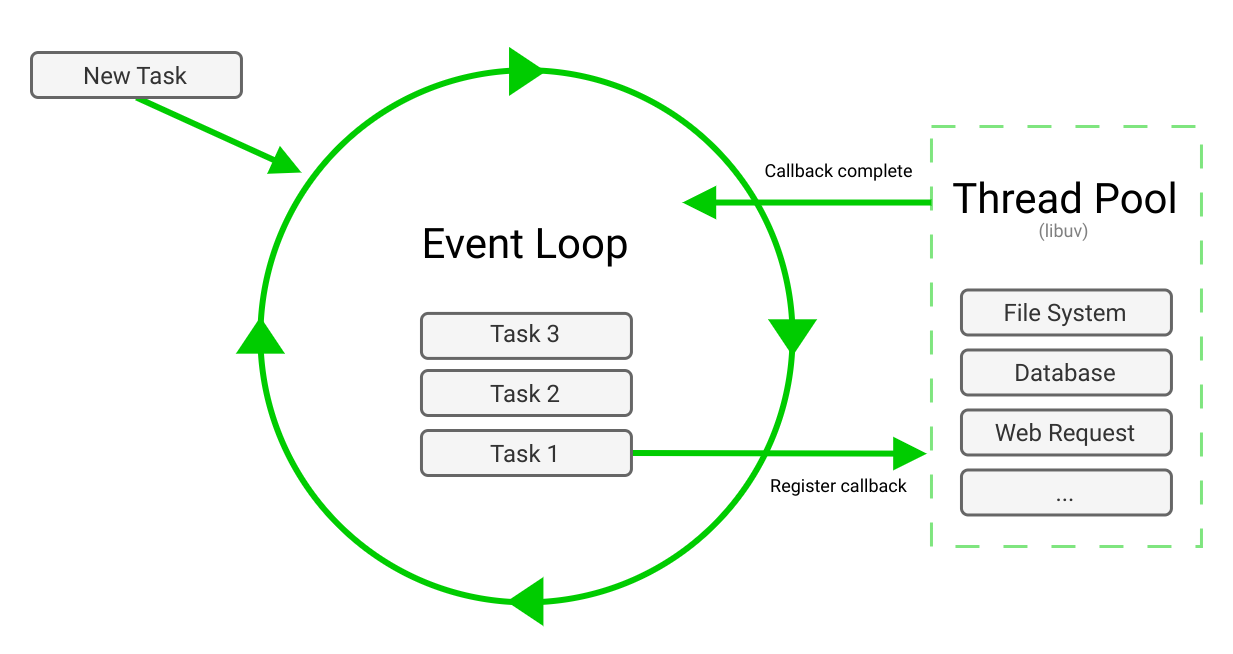
\includegraphics[width=.8\textwidth]{data/figures/nodejs.png}
    \fonte{Autor}
\end{figure}

Além disso, o NodeJS também dispõe do NPM, um gerenciador de pacotes reutilizáveis de código aberto, permitindo maior agilidade, flexibilidade e produtividade no processo de desenvolvimento \cite{npm2022}.